\documentclass[conference]{IEEEtran}

\usepackage[]{graphicx}    % We use this package in this document
\usepackage{amsmath}
\usepackage{mathtools}
\usepackage{subfiles}
\usepackage{amssymb}
\usepackage{hyperref}
\usepackage{algorithm}
\usepackage{algorithmic}
\usepackage{tikz,tikz-3dplot}
\usepackage{pgfplots}
\usepackage{subcaption}

\newcommand{\ignore}[1]{}  % {} empty inside = %% comment
\graphicspath{ {./pics/} }

\ifCLASSINFOpdf
\else
\fi

\hyphenation{op-tical net-works semi-conduc-tor}


\begin{document}
\onecolumn

\title{Heterogenous Autonomous Robotic Exploration (HARE)}

\author{Jackson~Parker}

% The paper headers
\markboth{IEEE JOURNAL XXXX, VOL. XX, NO. XX, MONTH 20XX}%
{Shell \MakeLowercase{\textit{et al.}}: Bare Demo of IEEEtran.cls for IEEE Journals}

% \markboth{IEEE JOURNAL OF SELECTED TOPICS IN APPLIED EARTH OBSERVATIONS AND REMOTE SENSING, VOL. XX, NO. XX, MONTH 20XX}



% If you want to put a publisher's ID mark on the page you can do it like
% this:
%\IEEEpubid{0000--0000/00\$00.00~\copyright~2015 IEEE}
% Remember, if you use this you must call \IEEEpubidadjcol in the second
% column for its text to clear the IEEEpubid mark.



% use for special paper notices
%\IEEEspecialpapernotice{(Invited Paper)}




% make the title area
\maketitle

% As a general rule, do not put math, special symbols or citations
% in the abstract or keywords.
\begin{abstract}
  The Heterogenous Autonomous Robotic Exploration system (HARE) is meant as a proof
  of concept for cooperative heterogenous systems that divide tasks based on the
  differentiable capabilities of the robots.
\end{abstract}

% Note that keywords are not normally used for peerreview papers.
\begin{IEEEkeywords}
IEEE, IEEEtran, journal, \LaTeX, paper, template.
\end{IEEEkeywords}


\IEEEpeerreviewmaketitle

\begin{figure}[H]
  \centering
    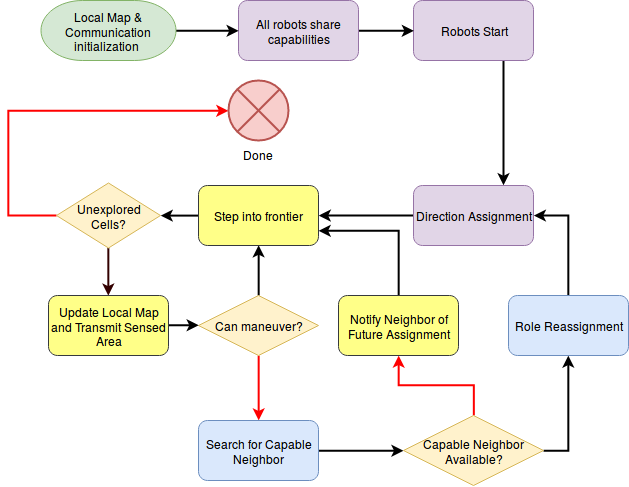
\includegraphics[width=0.5\textwidth]{HARE}
  \caption{High level block diagram for HARE}
  \label{fig:something3}
\end{figure}

%%%%%%%%%%%%%%%%%%%%%%%%%%%%%%%%%%%%%%
\section{Introduction}
%%%%%%%%%%%%%%%%%%%%%%%%%%%%%%%%%%%%%%
\subfile{tex/intro}

%%%%%%%%%%%%%%%%%%%%%%%%%%%%%%%%%%%%%%%%%%%
\section{Methodology}
%%%%%%%%%%%%%%%%%%%%%%%%%%%%%%%%%%%%%%%%%%%
\subfile{tex/methodology} %  <-- might be best to keep the example and remake some subfiles

%%%%%%%%%%%%%%%%%%%%%%%%%%%%%%%%%%%%%%%%%%%
\section{Results}
%%%%%%%%%%%%%%%%%%%%%%%%%%%%%%%%%%%%%%%%%%%
\subfile{tex/results} %  <-- might be best to keep the example and remake some subfiles

%%%%%%%%%%%%%%%%%%%%%%%%%%%%%%%%%%%%%%%%%%%
\section{Conclusion}
%%%%%%%%%%%%%%%%%%%%%%%%%%%%%%%%%%%%%%%%%%%
\subfile{tex/conclusion} %  <-- might be best to keep the example and remake some subfiles


% use section* for acknowledgment
\subfile{tex/appendix}
% \section*{Acknowledgment}

\ifCLASSOPTIONcaptionsoff
  \newpage
\fi



\bibliographystyle{IEEEtran}
% \bibliography{sources}
\bibliography{IEEEabrv,sources} % ftp://tug.ctan.org/pub/tex-archive/macros/latex/contrib/IEEEtran/bibtex/IEEEtran_bst_HOWTO.pdf


% insert where needed to balance the two columns on the last page with
% biographies
%\newpage

\begin{IEEEbiography}[{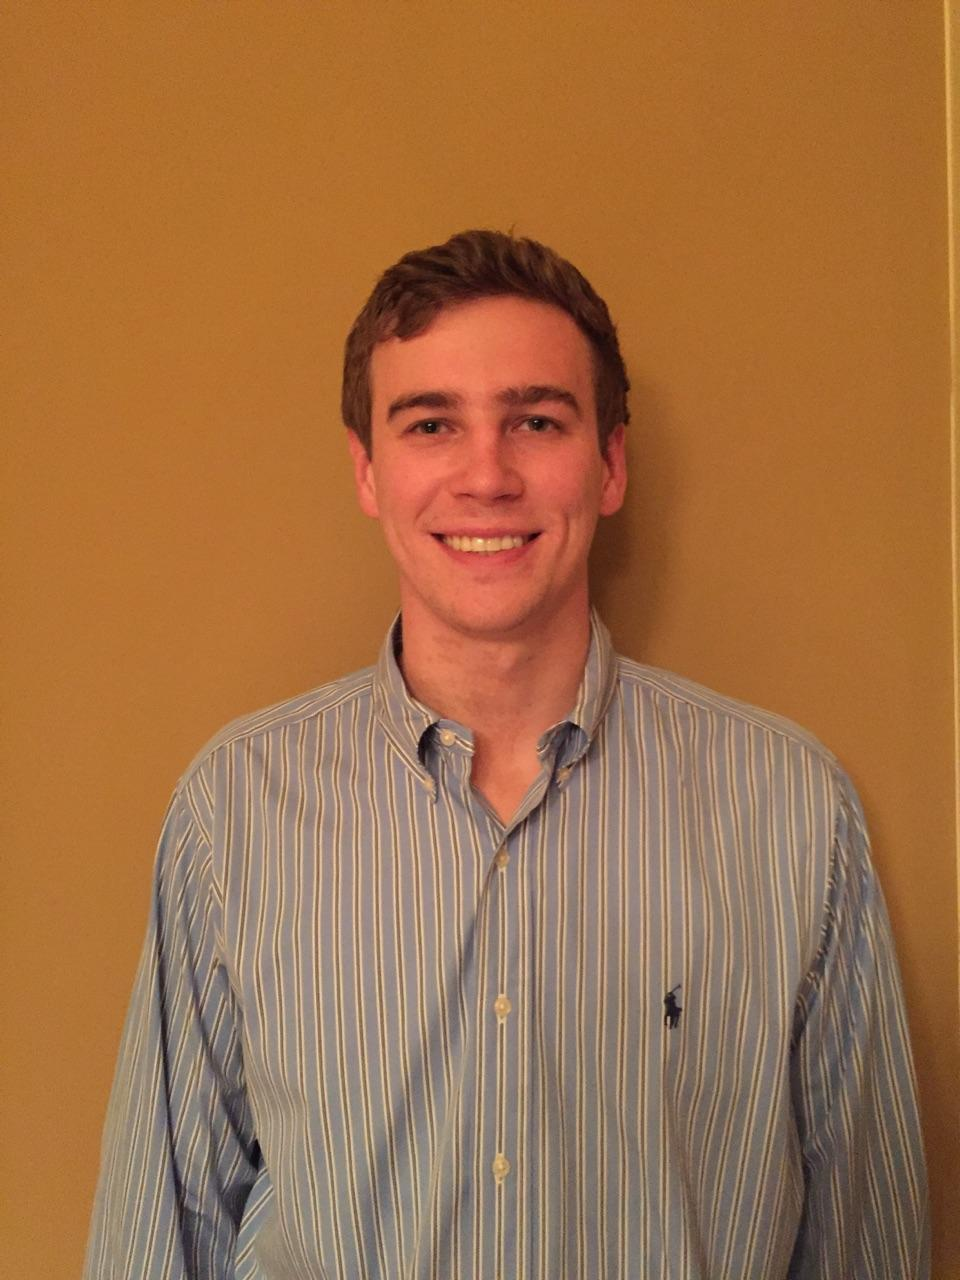
\includegraphics[width=1in,height=1.25in,clip,keepaspectratio]{pics/jackson_parker.jpeg}}]{Jackson Parker}
I work in the small satellite research lab as a systems engineer.
\end{IEEEbiography}



\end{document}
